\documentclass{article}

\usepackage[T1]{fontenc}

\usepackage{fancyhdr}
\usepackage{extramarks}
\usepackage{amsmath}
\usepackage{amsthm}
\usepackage{amsfonts}
\usepackage{tikz}
\usepackage{algorithm}
\usepackage{algpseudocode}
\usepackage{enumitem}

\usepackage[mono=false]{libertine}


\usetikzlibrary{automata,positioning}

%
% Basic Document Settings
%

\topmargin=-0.45in
\evensidemargin=0in
\oddsidemargin=0in
\textwidth=6.5in
\textheight=9.0in
\headsep=0.25in

\linespread{1.1}

\pagestyle{fancy}
\lhead{\hmwkAuthorName}
\chead{\hmwkClass: \hmwkTitle}
\rhead{\firstxmark}
\lfoot{\lastxmark}
\cfoot{\thepage}

\renewcommand\headrulewidth{0.4pt}
\renewcommand\footrulewidth{0.4pt}

\setlength\parindent{0pt}

%
% Create Problem Sections
%

\newcommand{\enterProblemHeader}[1]{
    \nobreak\extramarks{}{Problem \arabic{#1} continued on next page\ldots}\nobreak{}
    \nobreak\extramarks{Problem \arabic{#1} (continued)}{Problem \arabic{#1} continued on next page\ldots}\nobreak{}
}

\newcommand{\exitProblemHeader}[1]{
    \nobreak\extramarks{Problem \arabic{#1} (continued)}{Problem \arabic{#1} continued on next page\ldots}\nobreak{}
    \stepcounter{#1}
    \nobreak\extramarks{Problem \arabic{#1}}{}\nobreak{}
}

\setcounter{secnumdepth}{0}
\newcounter{partCounter}
\newcounter{homeworkProblemCounter}
\setcounter{homeworkProblemCounter}{1}
\nobreak\extramarks{Problem \arabic{homeworkProblemCounter}}{}\nobreak{}

%
% Homework Problem Environment
%
% This environment takes an optional argument. When given, it will adjust the
% problem counter. This is useful for when the problems given for your
% assignment aren't sequential. See the last 3 problems of this template for an
% example.
%
\newenvironment{homeworkProblem}[1][-1]{
    \ifnum#1>0
        \setcounter{homeworkProblemCounter}{#1}
    \fi
    \section{Problem \arabic{homeworkProblemCounter}}
    \setcounter{partCounter}{1}
    \enterProblemHeader{homeworkProblemCounter}
}{
    \exitProblemHeader{homeworkProblemCounter}
}

%
% Homework Details
%   - Title
%   - Due date
%   - Class
%   - Section/Time
%   - Instructor
%   - Author
%

\newcommand{\hmwkTitle}{Homework\ \#4}
\newcommand{\hmwkDueDate}{March 27, 2018}
\newcommand{\hmwkClass}{Design and Analysis of Algorithms}
\newcommand{\hmwkClassInstructor}{Professor Kasturi Varadarajan}
\newcommand{\hmwkAuthorName}{\textbf{Alic Szecsei}}

%
% Title Page
%

\title{
    \vspace{2in}
    \textmd{\textbf{\hmwkClass:\ \hmwkTitle}}\\
    \normalsize\vspace{0.1in}\small{Due\ in\ class\ on\ \hmwkDueDate}\\
    \vspace{0.1in}\large{\textit{\hmwkClassInstructor}}
    \vspace{3in}
}

\author{\hmwkAuthorName}
\date{}

\renewcommand{\part}[1]{\textbf{\large Part \Alph{partCounter}}\stepcounter{partCounter}\\}

%
% Various Helper Commands
%

% Useful for algorithms
\newcommand{\alg}[1]{\textsc{\bfseries \footnotesize #1}}

% For derivatives
\newcommand{\deriv}[1]{\frac{\mathrm{d}}{\mathrm{d}x} (#1)}

% For partial derivatives
\newcommand{\pderiv}[2]{\frac{\partial}{\partial #1} (#2)}

% Integral dx
\newcommand{\dx}{\mathrm{d}x}

% Alias for the Solution section header
\newcommand{\solution}{\textbf{\large Solution}}

% Probability commands: Expectation, Variance, Covariance, Bias
\newcommand{\E}{\mathrm{E}}
\newcommand{\Var}{\mathrm{Var}}
\newcommand{\Cov}{\mathrm{Cov}}
\newcommand{\Bias}{\mathrm{Bias}}

% Set from 1 to N
\newcommand{\XYZ}[1]{\left\{1,\ldots,{#1}\right\}}
\newcommand{\Break}{\textbf{break} }

\begin{document}

\maketitle

\pagebreak

\begin{homeworkProblem}

Consider the following randomized algorithm for generating biased random bits. The subroutine \alg{FairCoin} returns either 0 or 1 with equal probability; the random bits returned by \alg{FairCoin} are mutually independent.

\begin{algorithm}
	\begin{algorithmic}[1]
		\Function{OneInThree}{}
			\If{\Call{FairCoin}{} $= 0$}
				\State{\Return{0}}
			\Else
				\State{\Return{$1 - $\Call{OneInThree}{}}}
			\EndIf
		\EndFunction
	\end{algorithmic}
\end{algorithm}

\begin{enumerate}[label=(\alph*)]
	\item Prove that \alg{OneInThree} returns 1 with probability $\frac{1}{3}$.
	\item What is the \emph{exact} expected number of times that this algorithm calls \alg{FairCoin}?
	\item Now suppose you are \emph{given} a subroutine \alg{OneInThree} that generates a random bit that is equal to 1 with probability $\frac{1}{3}$. Describe a \alg{FairCoin} algorithm that returns either 0 or 1 with equal probability, using \alg{OneInThree} as your only source of randomness.
	\item What is the \emph{exact} expected number of times that your \alg{FairCoin} algorithm calls \alg{OneInThree}?
\end{enumerate}

\solution\\

\part

In order for \alg{OneInThree} to return 1, \alg{FairCoin} must return an odd number of 1s before returning a 0. We can begin to enumerate cases: first, that \alg{FairCoin} returns a 1 and then a 0 is $\frac{1}{2} \cdot \frac{1}{2} = \frac{1}{4}$. The probability that \alg{FairCoin} returns 3 1s and then a 0 is $\frac{1}{2} \cdot \frac{1}{2} \cdot \frac{1}{2} \cdot \frac{1}{2} = \frac{1}{16}$. The probability that \alg{FairCoin} returns 5 1s and then a 0 is $\frac{1}{2} \cdot \frac{1}{2} \cdot \frac{1}{2} \cdot \frac{1}{2} \cdot \frac{1}{2} \cdot \frac{1}{2} = \frac{1}{64}$, and so on. Our summation of all cases is then:
\begin{equation}
\frac{1}{4} + \frac{1}{16} + \frac{1}{64} + \ldots + \frac{1}{2^{2n}} = \sum_{k = 1}^{\infty} \frac{1}{2^{2k}}
\end{equation}

This is a geometric series with common ratio $r = \frac{1}{4}$; we can then use the formula $S = \frac{a_1}{1 - r}$ to determine the summation. Using this, we can see that $S = \frac{\frac{1}{4}}{1 - \frac{1}{4}} = \frac{\frac{1}{4}}{\frac{3}{4}} = \frac{1}{3}$. Therefore, \alg{OneInThree} has a $\frac{1}{3}$ probability of returning 1.\\

\part

Since \alg{OneInThree} might never terminate, our expected value of $T(n)$ is:
\begin{equation}
	E[T(n)] = \sum_{k = 1}^\infty k \cdot \text{Pr}[T(n) = k]
\end{equation}

In order for \alg{OneInThree} to terminate with exactly $k$ calls to \alg{FairCoin}, there must have been exactly $k-1$ times that \alg{FairCoin} returned 1 (and \alg{OneInThree} continued recursing), and 1 time it returned 0 (and \alg{OneInThree} stopped recursing). Thus, the combined probability for \alg{OneInThree} to terminate with exactly $k$ calls to \alg{FairCoin} is $\frac{1}{2^k}$. Plugging this back into our equation for $E[T(n)]$:

\begin{equation}
	\begin{split}
		E[T(n)] &= \sum_{k = 1}^\infty k \cdot \text{Pr}[T(n) = k]\\
		&= \sum_{k = 1}^\infty k \cdot \frac{1}{2^k}\\
		&= 2
	\end{split}
\end{equation}

\part

\begin{algorithm}
	\begin{algorithmic}[1]
		\Function{FairCoin}{}
			\State{$c_1 \gets \Call{OneInThree}{}$}
			\State{$c_2 \gets \Call{OneInThree}{}$}
			\If{$c_1 = 1$ and $c_2 = 1$}
				\State{\Return{\Call{FairCoin}{}}}
			\Else
				\If{$c_1 = 1$ or $c_2 = 1$}
					\State{\Return{$1$}}
				\Else
					\State{\Return{$0$}}
				\EndIf
			\EndIf
		\EndFunction
	\end{algorithmic}
\end{algorithm}

The idea for this algorithm is that we break the probability space into 3 partitions: first, the probability that both calls to \alg{OneInThree} return $1$ is $\frac{1}{9}$. The remaining probability is $\frac{8}{9}$; we further divide this into two partitions. The probability that both calls to \alg{OneInThree} returned $0$ is $\frac{4}{9}$; thus, the remaining probability (that only one call to \alg{OneInThree} returned $1$) is $\frac{4}{9}$.\\

Now, the probability that any call to \alg{FairCoin} which actually \emph{returns} will return 0 is clearly $\frac{1}{2}$; the same probability applies to any returning call to \alg{FairCoin} returning 1. Thus, \alg{FairCoin} has an equal probability of returning either 0 or 1.\\

\part

Since \alg{FairCoin} might never terminate, our expected value of $T(n)$ is:
\begin{equation}
	E[T(n)] = \sum_{k = 1}^\infty k \cdot \text{Pr}[T(n) = k]
\end{equation}

In order for \alg{FairCoin} to terminate with exactly $2k$ calls to \alg{OneInThree}, there must have been exactly $k-1$ times that both calls of \alg{OneInThree} returned 1 (and \alg{FairCoin} continued recursing), and 1 time at least one call returned 0 (and \alg{FairCoin} stopped recursing). Thus, the combined probability for \alg{FairCoin} to terminate with exactly $2k$ calls to \alg{FairCoin} is $\frac{1}{9^{k-1}} \cdot \frac{8}{9} = \frac{8}{9^k}$. Plugging this back into our equation for $E[T(n)]$:

\begin{equation}
	\begin{split}
		E[T(n)] &= \sum_{k = 1}^\infty 2k \cdot \text{Pr}[T(n) = k]\\
		&= \sum_{k = 1}^\infty 2k \cdot \frac{8}{9^k}\\
		&= \frac{9}{4}
	\end{split}
\end{equation}

\end{homeworkProblem}

\pagebreak

\begin{homeworkProblem}

Consider the following algorithm for finding the smallest element in an unsorted array:

\begin{algorithm}
	\begin{algorithmic}[1]
		\Function{RandomMin}{$A[1..n]$}
			\State{$min \gets \infty$}
			\For{$i \gets 1$ to $n$ in random order}
				\If{$A[i] < min$}
					\State{$min \gets A[i]$}\Comment{$(\star)$}
				\EndIf
			\EndFor
			\State{\Return{$min$}}
		\EndFunction
	\end{algorithmic}
\end{algorithm}

\begin{enumerate}[label=(\alph*)]
	\item In the worst case, how many times does \alg{RandomMin} execute line $(\star)$?
	\item What is the probability that line $(\star)$ is executed during the $n$th iteration of the for loop?
	\item What is the \emph{exact} expected number of executions of line $(\star)$?
\end{enumerate}

\solution\\

\end{homeworkProblem}

\pagebreak

\begin{homeworkProblem}

Suppose we have a circular linked list of numbers, implemented as a pair of arrays, one storing the actual numbers and the other storing successor pointers. Specifically, let $X[1..n]$ be an array of $n$ distinct real numbers, and let $N[1..n]$ be an array of indices with the following property: If $X[i]$ is the largest element of $X$, then $X[N[i]]$ is the smallest element of $X$; otherwise, $X[N[i]]$ is the smallest among the set of elements in $X$ larger than $X[i]$. For example:

\begin{table}[h]
	\centering
		\begin{tabular}{r | *{9}{c} }
			$i$    &  1 &  2 &  3 &  4 &  5 &  6 &  7 &  8 &  9 \\
			\hline
			$X[i]$ & 83 & 54 & 16 & 31 & 45 & 99 & 78 & 62 & 27 \\
			\hline
			$N[i]$ &  6 &  8 &  9 &  5 &  2 &  3 &  1 &  7 &  4
		\end{tabular}
\end{table}

Describe and analyze a randomized algorithm that determines whether a given number $x$ appears in the array $X$ in $O(\sqrt{n})$ expected time. \emph{\textbf{Your algorithm may not modify the arrays $X$ and $N$.}}\\

\solution\\

\end{homeworkProblem}

\pagebreak

\begin{homeworkProblem}

A \emph{majority tree} is a complete binary tree with depth $n$, where every leaf is labeled either 0 or 1. The \emph{value} of a leaf is its label; the \emph{value} of any internal node is the majority of the values of its three children. Consider the problem of computing the value of the root of a majority tree, given the sequence of $3^n$ leaf labels as input. For example, if $n = 2$ and the leaves are labeled 1, 0, 0, 0, 1, 0, 1, 1, 1, the root has value 0.

\begin{figure}[h]
	\centering
		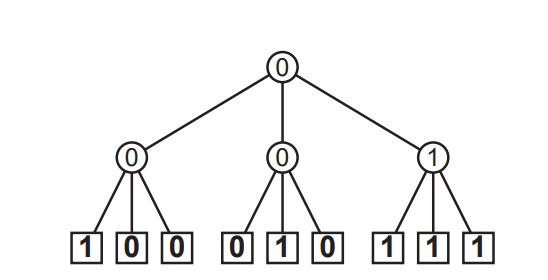
\includegraphics{images/majoritytree.png}
	\caption{A majority tree with depth $n = 2$.}
	\label{fig:majoritytree}
\end{figure}

\begin{enumerate}[label=(\alph*)]
	\item Prove that \emph{any} deterministic algorithm that computes the value of the root of a majority tree \emph{must} examine every leaf. \emph{[Hint: Consider the special case $n = 1$. Recurse.]}
	\item Describe and analyze a randomized algorithm that computes the value of the root in worst-case expected time $O(c^n)$ for some constant $c < 3$. \emph{[Hint: Consider the special case $n = 1$. Recurse.}
\end{enumerate}

\solution\\

\end{homeworkProblem}

\pagebreak

\begin{homeworkProblem}

Suppose you are given a graph $G$ with weighted edges, and your goal is to find a cut whose total weight (not just number of edges) is smallest.

\begin{enumerate}[label=(\alph*)]
	\item Describe an algorithm to select a random edge of $G$, where the probability of choosing edge $e$ is proportional to the weight of $e$.
	\item Prove that if you use the algorithm from part (a), instead of choosing edges uniformly at random, the probability that \alg{GuessMinCut} returns a minimum-weight is still $\Omega(1/n^2)$.
	\item What is the running time of your modified \alg{GuessMinCut} algorithm?
\end{enumerate}

\solution\\

\end{homeworkProblem}

\end{document}